\documentclass[aspectratio=169,12pt]{beamer}
\usepackage{amsmath}
\usepackage{amssymb}
\usepackage[most]{tcolorbox}
\usepackage{tikz}
\usepackage{graphicx}
\usepackage[sfdefault,lf]{FiraSans}
\renewcommand{\familydefault}{\sfdefault}
\setlength{\parindent}{0pt}
\everymath{\displaystyle}

\setbeamertemplate{navigation symbols}{}
\setbeamertemplate{footline}{}
\setbeamertemplate{headline}{}

\definecolor{mmpageWhite}{HTML}{FCFBF7}
\definecolor{mmtanSoft}{HTML}{F7F5EF}
\definecolor{mmgreenDeep}{HTML}{244B2C}
\definecolor{mmgreenLeaf}{HTML}{5D8A56}
\definecolor{mmgreenSoft}{HTML}{E4EFD9}
\definecolor{mmtext}{HTML}{163221}

\setbeamercolor{background canvas}{bg=mmpageWhite}
\setbeamercolor{normal text}{fg=mmtext,bg=mmpageWhite}

\newtcolorbox{MMProblemCard}[1][]{enhanced,breakable=false,colback=white,colframe=black,boxrule=1.5pt,arc=8pt,left=5pt,right=5pt,top=4pt,bottom=4pt,before skip=0pt,after skip=0pt,height=0.245\textheight,valign=top,#1}
\newcommand{\KoruIcon}{\raisebox{-0.2em}{
\includegraphics[height=1.05em]{../../SITE/header-logo.png}}}
\newcommand{\HoeIcon}{\raisebox{-0.2em}{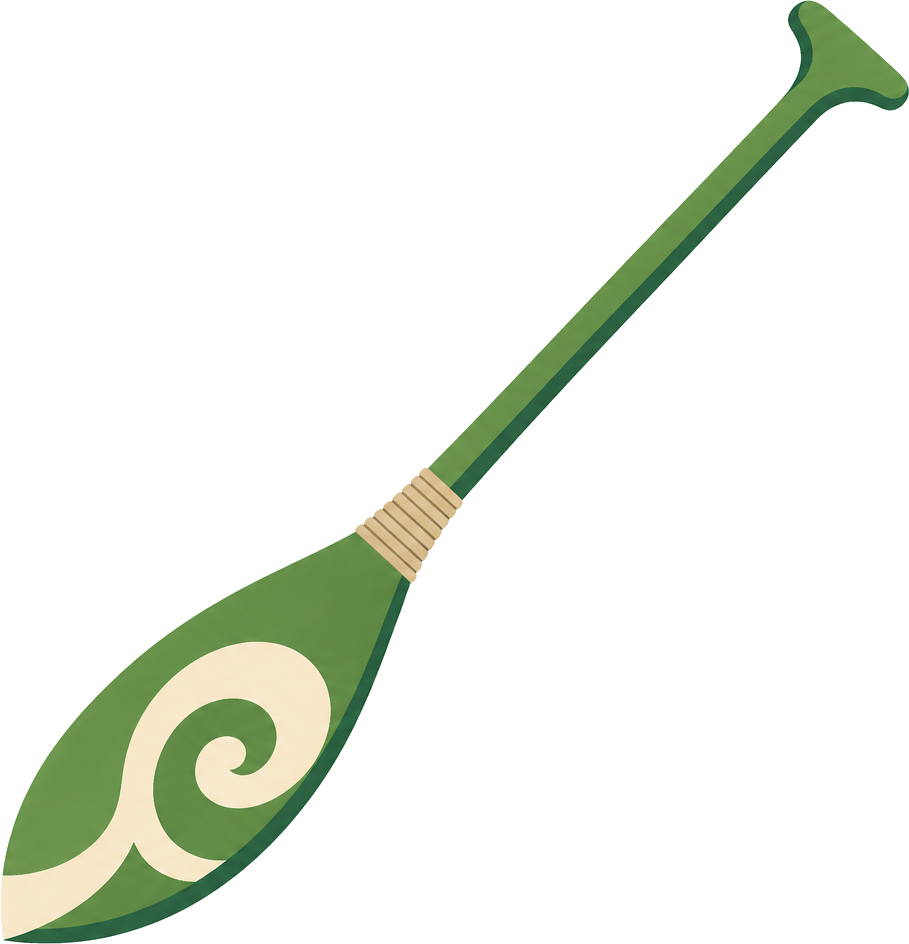
\includegraphics[height=1.05em]{../../SITE/hoe.png}}}
\newcommand{\ScaffoldIcons}[1]{\ifcase#1\or \HoeIcon\or \HoeIcon\hspace{0.22em}\KoruIcon\or \KoruIcon\hspace{0.22em}\KoruIcon\hspace{0.22em}\KoruIcon\fi}
\newcommand{\WorksheetTitle}[2]{%
  {\colorbox{mmtanSoft}{\parbox[c][2.0em][c]{0.975\linewidth}{%
    \hspace{0.25em}{\Large\bfseries\textcolor{mmgreenDeep}{#1}\hfill\ScaffoldIcons{#2}}}}
  \par\vspace{0.08em}{\color{mmgreenLeaf}\rule{\linewidth}{2.0pt}}\par\vspace{0.04em}}
}
\newcommand{\MMProblem}[2]{\begin{MMProblemCard}\raggedright\small\textbf{#1.} #2\par\end{MMProblemCard}}

\setbeamertemplate{background}{
 \begin{tikzpicture}[remember picture,overlay]
 \draw[black,line width=1.5pt,rounded corners=10pt]
 ([xshift=0.45cm,yshift=-0.45cm]current page.north west)
 rectangle
 ([xshift=-0.45cm,yshift=0.45cm]current page.south east);
 \end{tikzpicture}
}

% Default worksheet generation rules:
% use notes-style beamer pages
% use bordered cards for individual problems
% target 9 problems per frame in a 3x3 grid
% target 3 frames per scaffold by default where content allows

\begin{document}\begin{frame}[t]
\WorksheetTitle{Push Tasks}
\vspace{-0.18em}
\begin{columns}[T,onlytextwidth]
\begin{column}{0.32\textwidth}\MMProblem{1}{A circle's area is \mbox{$36\pi$} cm\mbox{$^2$}. Find its circumference in terms of \mbox{$\pi$}.}\end{column}
\begin{column}{0.32\textwidth}\MMProblem{2}{A circle's circumference is \mbox{$20\pi$} m. Find its area in terms of \mbox{$\pi$}.}\end{column}
\begin{column}{0.32\textwidth}\MMProblem{3}{The area of a circle is increased by 44\%. By what percentage does its radius increase?}\end{column}
\end{columns}
\vspace{0.45em}
\begin{columns}[T,onlytextwidth]
\begin{column}{0.32\textwidth}\MMProblem{4}{The circumference of a circle is tripled. By what factor does its area increase?}\end{column}
\begin{column}{0.32\textwidth}\MMProblem{5}{A square and a circle have the same perimeter. If the square has side length 11 cm, find the area of the circle.}\end{column}
\begin{column}{0.32\textwidth}\MMProblem{6}{A rectangle has length 12 cm and width equal to the diameter of a circle with area \mbox{$25\pi$} cm\mbox{$^2$}. Find the rectangle's perimeter.}\end{column}
\end{columns}
\vspace{0.45em}
\begin{columns}[T,onlytextwidth]
\begin{column}{0.32\textwidth}\MMProblem{7}{Find the area of the shaded region when a circle of radius 10 cm has a square of side length 14 cm inscribed in it.}\end{column}
\begin{column}{0.32\textwidth}\MMProblem{8}{Four semicircles of diameter 8 cm are arranged to form a shape. Find the total perimeter of the shape.}\end{column}
\begin{column}{0.32\textwidth}\MMProblem{9}{A circular sector has radius 15 cm and central angle \mbox{$72^\circ$}. Find its arc length and area.}\end{column}
\end{columns}
\end{frame}
\begin{frame}[t]
\WorksheetTitle{Push Tasks}
\vspace{-0.18em}
\begin{columns}[T,onlytextwidth]
\begin{column}{0.32\textwidth}\MMProblem{1}{Two concentric circles have radii 7 cm and 10 cm. Find the area of the annulus (ring) between them.}\end{column}
\begin{column}{0.32\textwidth}\MMProblem{2}{A wire is bent to form a circle of radius 21 cm. The same wire is then bent to form a square. Find the area of the square.}\end{column}
\begin{column}{0.32\textwidth}\MMProblem{3}{A circular flower bed has circumference 31.4 m. A path 1 m wide is built around it. Find the area of the path.}\end{column}
\end{columns}
\vspace{0.45em}
\begin{columns}[T,onlytextwidth]
\begin{column}{0.32\textwidth}\MMProblem{4}{The ratio of the areas of two circles is 9:16. If the smaller circle has circumference \mbox{$18\pi$} cm, find the radius of the larger circle.}\end{column}
\begin{column}{0.32\textwidth}\MMProblem{5}{A running track consists of two straight sections each 100 m long and two semicircular ends. If the total length of the track is 400 m, find the area enclosed by the track.}\end{column}
\begin{column}{0.32\textwidth}\MMProblem{6}{A circle is inscribed in a square of side length 14 cm. Find the area of the region outside the circle but inside the square.}\end{column}
\end{columns}
\vspace{0.45em}
\begin{columns}[T,onlytextwidth]
\begin{column}{0.32\textwidth}\MMProblem{7}{A goat is tied to a corner of a square shed with side length 10 m. The rope is 15 m long. Find the area the goat can graze (outside the shed).}\end{column}
\begin{column}{0.32\textwidth}\MMProblem{8}{Find the radius of a circle whose area is equal to the sum of the areas of two circles with radii 6 cm and 8 cm.}\end{column}
\begin{column}{0.32\textwidth}\MMProblem{9}{A circular pizza is cut into 8 equal slices. If the diameter is 40 cm, find the perimeter of one slice (including the two straight edges).}\end{column}
\end{columns}
\end{frame}
\begin{frame}[t]
\WorksheetTitle{Push Tasks}
\vspace{-0.18em}
\begin{columns}[T,onlytextwidth]
\begin{column}{0.32\textwidth}\MMProblem{1}{The minute hand of a clock is 12 cm long. Find the area swept by the minute hand in 25 minutes.}\end{column}
\begin{column}{0.32\textwidth}\MMProblem{2}{A circular pond has diameter 8 m. A concrete path 2 m wide is built around it. Find the cost of concreting the path at \$\mbox{$45$} per m\mbox{$^2$}.}\end{column}
\begin{column}{0.32\textwidth}\MMProblem{3}{}\end{column}
\end{columns}
\vspace{0.45em}
\begin{columns}[T,onlytextwidth]
\begin{column}{0.32\textwidth}\MMProblem{4}{}\end{column}
\begin{column}{0.32\textwidth}\MMProblem{5}{}\end{column}
\begin{column}{0.32\textwidth}\MMProblem{6}{}\end{column}
\end{columns}
\vspace{0.45em}
\begin{columns}[T,onlytextwidth]
\begin{column}{0.32\textwidth}\MMProblem{7}{}\end{column}
\begin{column}{0.32\textwidth}\MMProblem{8}{}\end{column}
\begin{column}{0.32\textwidth}\MMProblem{9}{}\end{column}
\end{columns}
\end{frame}
\end{document}
